\documentclass{beamer}

\usetheme{Warsaw}
\usepackage{graphicx}
% include.tex
\newcommand{\Bernoulli}[1]{\text{Bernoulli} \left( #1 \right)}
\newcommand{\mydigamma}[1]{\psi \left( #1 \right)}
%\newcommand{\diag}[1]{\text{diag}\left( #1 \right)}
\newcommand{\tr}[1]{\text{tr}\left( #1 \right)}
\newcommand{\Poisson}[1]{\text{Poisson} \left( #1 \right)}
\def \half {\frac{1}{2}}
\def \R {\mathbb{R}}
\def \vbeta {\vec{\beta}}
\def \vy {\vec{y}}
\def \vmu {\vec{\mu}}
\def \vmuqbeta {\vmu_{q(\vbeta)}}
\def \vmubeta {\vmu_{\vbeta}}
\def \Sigmaqbeta {\Sigma_{q(\vbeta)}}
\def \Sigmabeta {\Sigma_{\vbeta}}
\def \va {\vec{a}}
\def \vtheta {\vec{\theta}}
\def \mX {\vec{X}}

\def\ds{{\displaystyle}}

\def\diag{{\mbox{diag}}}


\title{Zero-inflated models}
\author{Mark Greenaway}

\mode<presentation>
{ \usetheme{boxes} }

\begin{document}
% 1. Front slide
\begin{frame}
\titlepage
% Details about myself here?
\end{frame}

% 2. Intro
\begin{frame}
\frametitle{Introduction}
Zero inflated data arises in many areas of application, such as physical
activity data, number of hospital visits and number of insurance claims per
year.

We will work with zero-inflated count data. I encountered this sort of data while
analysing the data arising from the Get Healthy project.
\end{frame}
% 3. Univariate model
\begin{frame}
\frametitle{Univariate model formulation}
We start by building a relatively simple zero-inflated count model.

\begin{align*}{ll}
X_i &= R_i Y_i \\
R_i &\sim \text{Bernoulli}(\rho) \\
Y_i &\sim \text{Poisson}(\lambda) \\
\rho &\sim \text{Beta}(a_\rho, b_\rho) \\
\lambda &\sim \text{Gamma}(a_\lambda, b_\lambda)
\end{align*}

\end{frame}

% 4. \rho = 9/10, \lambda = 5
% Example data 0 0 0 5 10
\begin{frame}[fragile]
\frametitle{Example data}
Take, for example, $\rho = \frac{1}{2}, \lambda = 5$.

\begin{verbatim}
0 7 3 4 5 3 2 6 5 0 0 1
0 0 5 0 2 3 6 4 0 5 4 0
7 0 0 0 7 0 6 6 0 3 0 5
0 4 0 0 0 2 3 0 3 4 5 0
8 0
\end{verbatim}

% Histogram
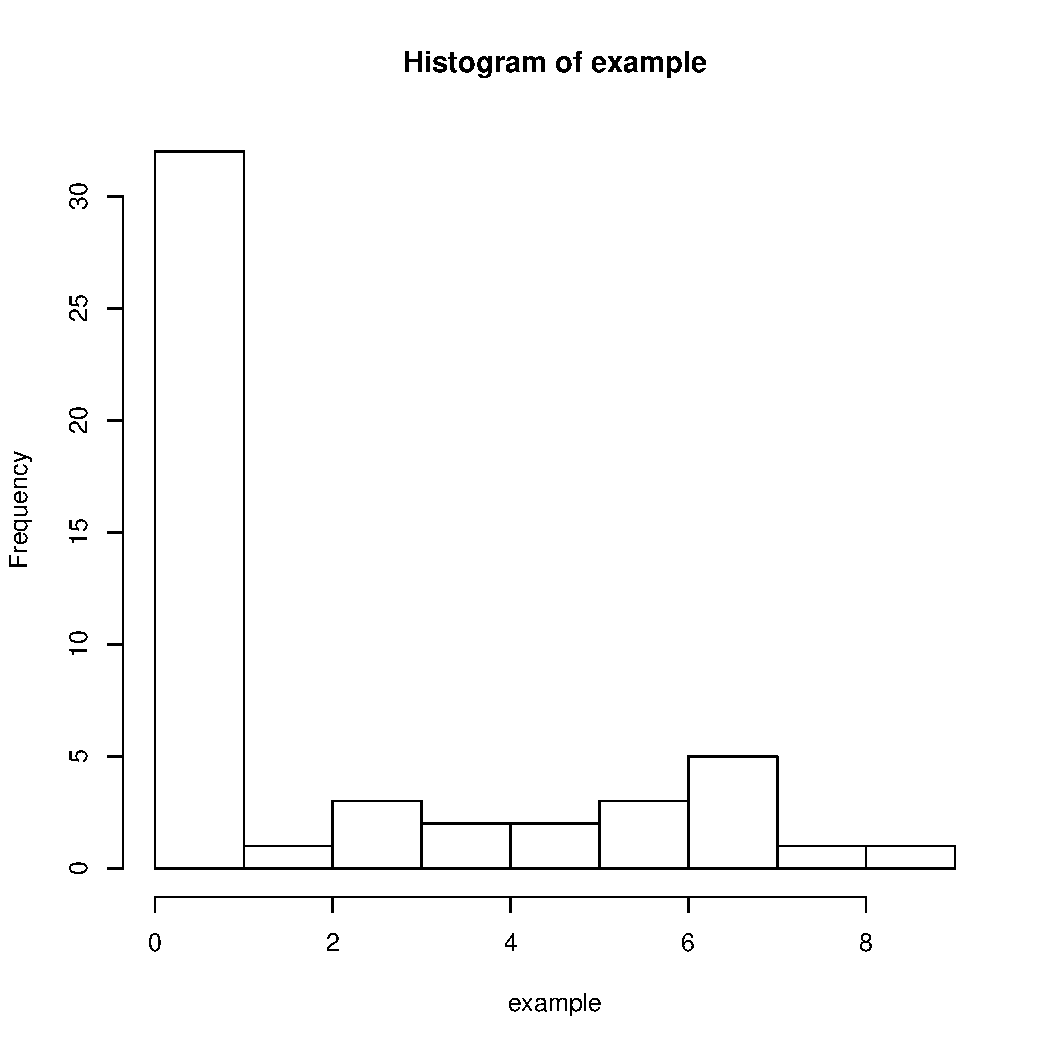
\includegraphics[width=50mm, height=50mm]{code/univariate_data_histogram.pdf}
% Density
\end{frame}

% 5. How to fit, and advantages and disadvantages of each approach
% - Maximum likelihood
% - MCMC
% - VB
\
\begin{frame}
\frametitle{Comparison of fitting techniques}
\begin{tabular}{p{2cm}p{3.75cm}p{3.75cm}}
Technique & Pro & Con \\
\hline
MLE & Standard optimisation techniques can be used & Biased for mixed models \\
& & \\ %Frequentist \\
\hline
MCMC & Bayesian & Slow \\
	& Very accurate &  May not converge at all \\
\hline
Variational Bayes & Bayesian & May lose accuracy, or underestimate variance \\
& Fast  & Solution may be intractable \\ 
& Still quite accurate & \\
\hline
\end{tabular}

\end{frame}

% 6. Overview of Variational Bayes
\begin{frame}
\frametitle{An overview of Variational Bayes}
\begin{itemize}
\item Approximate the full posterior $p(\theta)$ with an approximation $q(\theta)$
\item Minimise the KL divergence between $p(\theta)$ and $q(\theta)$
\item Theory guarantees that $q(\theta) < p(\vx, \theta)$ and that $q(\theta)$ will
increase with each VB step
\end{itemize}
\end{frame}

% 7a. Variational Bayes solution to ZIP
% - q-densities
\begin{frame}
Choose a factored approximation of the form
$$
q(\theta) = q(\lambda) q(\rho) \prod_{i=1}^n q(r_i)
$$
where
\begin{align*}{ll}
q(\lambda) &= \text{Gamma}(a_{q(\lambda)}, b_{q(\lambda)}) \\
q(\rho) &= \text{Beta}(a_{q(\rho)}, b_{q(\rho)}) \\
q(r_i) &= \text{Bernoulli}(p_i)
\end{align*}

% - Algorithm
We iteratively update the parameters of each approximate distribution
in turn until the lower bound of the approximation converges.

This could be thought of as a generalisation of Expectation Maximisation.
\end{frame}


% 8. Results
% - Lower bound convergence
% - Accuracies
% 7b. Define accuracy
\begin{frame}
\frametitle{Mean field updates}
% Are they going to be happy with that?
As we are using conjugate priors in our model, the mean field updates can be derived.
\begin{align*}{ll}
q(\lambda) &= \text{Gamma}(\alpha_\lambda + \vone^T \vx, \beta_\lambda + \vone^T\vp) \\
q(\rho) &= \text{Beta}(\alpha_\rho + \vone^T\vr, \beta_\rho + \vone^T(\vone - \vr)) \\
q(r_i) &= \text{Bernoulli}(\text{expit}(\eta_i))
\end{align*}
where
$$
\eta_i = - \frac{\alpha_{q(\lambda)}}{\beta_{q(\lambda)}} + \Psi(\alpha_{q(\rho)}) - \Psi(\beta_{q(\rho)})
$$
\end{frame}

\begin{frame}
\frametitle{Results/Accuracy}
% Definition of accuracy
Accuracy is defined as the difference in $L_1$ norm between the true posterior distribution and
the approximate posterior distribution of the variational approximation.

Excellent accuracy for the univariate approximation, over 99\% in all of the cases that I looked at.
% Graph of lower bound
%\includegraphics{univariate_lower_bound_convergence.pdf}
\end{frame}

% 9. Extension to linear model
% 10. Overview GVA
% 11. Algorithm
% 12. Results?
% 13. What next
% 14. Conclusion
% 15. References
\begin{frame}
\frametitle{Extension to multivariate/regression models}
Extension from univariate, model formulation
$$
q(\theta) = q(\beta) q(\rho) \prod_{i=1}^n q(r_i)
$$
where
$q(\beta) \sim N(\mu, \Sigma)$ and
$q(\sigma_u^2) \sim IG(\alpha_{\sigma_u^2}, \beta_{\sigma_u^2})$

\begin{itemize}
\item Mixed models -- Applied statisticians love these.
\item There is a need for better approaches to fitting zero-inflated mixed models.
\item For example, MCMC with existing software can take minutes to
converge, or not converge at all.
\item That might not sound so bad to you, but how do you
do model selection? Applied statisticians and biostatisticians rarely know the true model
\end{itemize}
\end{frame}

\begin{frame}
\frametitle{Gaussian and Laplacian Variational Approximations}
\begin{itemize}
\item Lack of conjugacy means mean field updates won't be analytically tractable for the regression parameters.
\item We try Gaussian Variational Approximations instead, assuming that
$$
\begin{pmatrix}
\beta \\
\vu
\end{pmatrix}
\sim N(\vmu, \Sigma)
$$
and approximate as closely as we can
\item For each iteration, we use Newton-Raphson style optimisation to find
$$
\begin{pmatrix}
\beta \\
\vu
\end{pmatrix}
$$
and then perform mean field updates on the other parameters
\item Computation - a work in progress
\item Initial signs are that this approach will work. The correct parameters are estimated for simulated test cases
that we have tried.
\end{itemize}
\end{frame}

\begin{frame}
\frametitle{References}
\begin{itemize}
\item Explaining variational approximations, J. T. Ormerod, M. P. Wand, American Statistician, 2010
\item Gaussian Variational Approximations, J. T. Ormerod, M. P. Wand, 2012
\item General Design Mixed Models, J. T. Ormerod, M. P. Wand, 2006
\end{itemize}
\end{frame}

\end{document}
